\chapter{Image Acquisition and Calibration}

As mentioned in the system architecture, images need to be taken simultaneously. There also needs to be two cameras due to the way the cameras are constructed, with a Bayer matrix (See intrinsic parameters) for each pixel. At the time of inception, one could only isolate NIR from RGB using separate cameras. Attempts to have both on a single camera were ineffective (explain why).\\

The

\section{Review of concepts}

These concepts are crucial to understand the reasoning behind certain decisions.

\subsection{Intrinsic Parameters}

focal length

\subsection{Distortion}

(picture of distortion)

\subsubsection{Bayer matrix}

\subsection{Extrinsic Parameters}

translation, rotation, sun, glare

\subsection{Camera Calibration}

(picture of undistortion).

\subsubsection{Jello effect}

ripple

\section{Filters}

A filter is needed to isolate the NIR channel. If a custom filter is used on a camera with the NIR filter removed, it is possible to isolate a NIR channel without visible light leakage on one or more colour channels. Variants include the Wratten 25A Red Long Pass filter, the Wratten 87 NIR All Pass filter and the Rosco 2008 Blue filter, which allow red and NIR light, only NIR light, and blue and NIR light respectively.\\

The Rosco 2008 Blue filter will be used, for most of the project, as well as the 600nm Dichroic Glass Longpass filter and 500nm Dichroic Glass Bandpass filter from Edmund Scientific, with limited access.

The blue Rosco 2008 filter is used as in Figure \ref{fig:blue_filter}, and passes only NIR within the green and red channels, as shown in Figure \ref{fig:blue_curve}.

\begin{figure}[H]
\begin{subfigure}{0.5\textwidth}
\centering
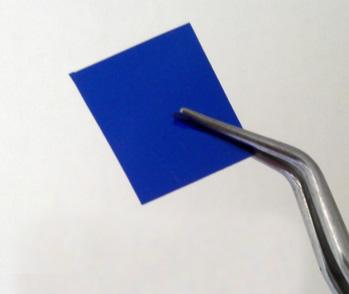
\includegraphics[scale=0.45]{images/blue_filter.jpg}
\caption{Blue Rosco 2008 filter \cite{blue_filter}}
\label{fig:blue_filter}
\end{subfigure}
\begin{subfigure}{0.5\textwidth}
\centering
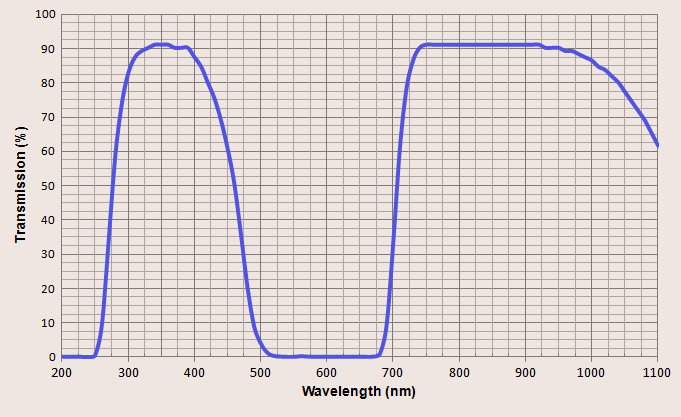
\includegraphics[scale=0.42]{images/superblueinfraredfiltercurve.png}
\caption{Blue filter transmission curve.}
\label{fig:blue_curve}
\end{subfigure}
\caption{Blue filter characteristics \cite{blue_curve}}
\label{fig:blue_character}
\end{figure}

\section{Cameras}

Two cameras are required. It is seemingly impossible to capture pure NIR and pure red on separate channels unless the intrinsic bayer matrix (see chapter 4 on intrinsic parameters) is manufactured to allow for it, however, then it would not be cost effective (citation needed).\\

The Sony IMX219 series cameras will be used. They integrate with the Raspberry Pi using a single 15-pin CSI connection.

\section{Camera mount}

The cameras will be fixed relative to each other using a PCB substrate so that no rotational or translational drift can occur.

Also, the cameras are to be dampened to prevent a jello-effect due to the rolling shutter cameras. Global shutter cameras are more expensive.

Ripple / jello

Thus, a DC brushless motorised gimbal will not be necessary.

\section{Simultaneous triggering}

A few solutions will be investigated, including the use of TCP/UDP packets and 'on the second' triggering.

Initially TCP triggering was used, but the overhead and asynchronous nature meant that it was never consistently triggered at the same time. Instead, the clocks are sychronised using NTP, and attempt to trigger every second, on the second. The latter solution works quite well, with an occassional few milliseconds difference in stereo captures.

\section{Calibration}

Stereo-calibration using 16x16 square chess board images were used.

\subsection{Calibration Technique}

\subsection{Measured Results}

\section{Stereo-rectification}

The images were undistorted (see chapter 4 on intrinsic parameters) according to the simultaneous chess board images it was calibrated at.

\subsection{Measured Results}